\documentclass[a4paper]{article}

\setlength{\oddsidemargin}{-4mm}
\addtolength{\topmargin}{-1in}
\addtolength{\footskip}{+0.5in}
\addtolength{\textwidth}{+1.5in}
\addtolength{\textheight}{+1in}

\usepackage[utf8]{inputenc}
\usepackage[english]{babel}
\usepackage{listings}
\usepackage{color}
\usepackage{multirow}
\usepackage{rotating}
\usepackage{graphicx}
\usepackage{caption}
\usepackage{amsmath}

\renewcommand{\familydefault}{cmr}

\title{Report of Click Labs}
\author{Hong-Nam Hoang, Manh-Ha Nguyen and Xuan-Thu Thi Le}
\date{\today}

\begin{document}

  \maketitle

  \definecolor{stringcolor}{rgb}{0.20,0.50,0.20}
  \definecolor{commentcolor}{rgb}{0.40,0.40,0.40}
  \definecolor{keywordcolor}{rgb}{0.50,0.10,0.10}
  \definecolor{idcolor}{rgb}{0.10,0.10,0.50}
  \definecolor{bg}{rgb}{0.95,0.95,0.95}  
  \lstdefinestyle{C}{basicstyle=\ttfamily,
                          keywordstyle=*\color{keywordcolor}\bfseries,
                          identifierstyle=\color{idcolor},
                          commentstyle={\color{black}\it},
                          stringstyle={\color{stringcolor}\ttfamily},
                          showstringspaces=false,
                          breaklines=true,
                          numbers=left,
                          numbersep=10pt,
                          stepnumber=1,
                          numberstyle=\small,
                          frame=single,
                          }

  \lstdefinelanguage[]{Click}[]{SQL}{
    morekeywords={elementclass, Counter, InfiniteSource, RateSource, Print, Paint, PaintSwitch, Script}}

  \section{Introduction}
  \section{ClickLabs package}
    \subsection{File organization}
      \begin{description}
      	\item[elements/] This directory contains all the additional click elements using in the lab.
      	\item[plot-template/] This directory contains templates used for plotting data by gnuplot. These files are used by draw-graph.sh
      	\item[bin/update-elements.sh] Run this file to update the new elements implemented in directory elements (above). For more information, type: ./update-elements.sh -h
      	\item[bin/visual-clicky.sh]Shell script to visualize click experiment using clicky. For more information, type: ./visual-clicky.sh -h
      	\item[bin/init.sh]Initialize Click environment for lab. Just run init.sh in the first time you get this source or click source directory changed.
      	\item[bin/eclick-compile.sh] Extend the Click file. A click file can include another one to reuse some compound elements (similar include in C, or import in Java). File eclick-compile.sh is used to translate (or flatten) these extended-click file to a normal click file.
      	\item[bin/convert-click-dump.sh]This script used to transform dump files from click (binary files) into text files. Note: this is one-way transformation, the binary files cannot be recovered from the text files.
      	\item[bin/draw-graph.sh] This script is used to draw graphs from data extracted in CLICK dump files. Just provide the dump files, this script will generate a graph for you. Note: No need to use convert-click-dump.sh before using draw-graph.sh.
      	\item[bin/draw-graph-framerelay.sh] Based on draw-graph.sh, this script helps to show the characteristics of verifying a conformant flow (which is deal with CIR, CBS, EBS).
      	\item[clicky.ccss] File supporting Clicky Cascading Style Sheets. It controls the appearance of a Clicky diagram with style sheets written in a CSS-like language.      	
      	\item[1-test-config/]
      	\item[2-tcp-udp-generation/]
      	\item[3-shaper-policer/]
      	\item[4-scheduler/]
      \end{description}
    
    \subsection{Some introductions before surfing click configurations}
      \begin{enumerate}
      	\item 
      	  First of all, initialize the click environment for these stuffs. Run file init.sh: \\
      	    \texttt{chmod +x init.sh\\
      	    ./init.sh}\\
      	  Normally, init process takes long time for the first finding Click source
  path. To save time, you can create file $~/.clickrc$ with the content similar
  to this:\\
            \texttt{export CLICK\_SRC=/home/iizke/click/click-1.8.0}
        
        \item 
          While finishing to code some Click elements, put it in directory 'elements', and then run file update-elements.sh to compile and install new elements: \\
    \texttt{chmod +x update-elements.sh\\
    update-elements.sh}
        \item
        Explore the click configuration by using tool visual-clicky.sh. Simple way to use: \\    
    \texttt{visual-clicky.sh \$CLICK\_CONFIGURATION\_FILE}
        \item
        To support easy-reading and team-working activities, we developed a tool to allow including some click files into a click file. If you write some click files as library files, you can reuse it by using 'include statement'. For example, we have TCP\_Source.click to implement a TCP-generator, and UDP\_Source.click to implement an UDP-generator. In TCP\_UDP.click, we reuse the implementation of these generator by adding these lines at anywhere in TCP\_UDP.click file (but should be in the top for easy reading): \\
        \texttt{
  ------------------------ file: TCP\_UDP.click ---------------------------\\
  //#include "TCP\_Source.click"\\
  //#include "UDP\_Source.click"\\
  ...\\
  --------------------------------------------------------------------------}\\
  The syntax of include statement is simple:\\
          \texttt{//#include "CLICK\_PATH"}\\
  where CLICK\_PATH can be relative or absolute path. After that, you have to use our tool (eclick-compile.sh) to precompile this file before simulating it by CLICK, for example:\\
    eclick-compile.sh -o extend-TCP\_UDP.click [-f] TCP\_UDP.click\\
Note: if using tool visual-clicky.sh, you don't have to pre-compile the extended-click file. It will do automatically.
        \item
        \begin{flushleft}
        To visualize your packet stream at input or output, we have developed draw-graph.sh to generate graph as picture (using gnuplot). So, before using this function, make sure that you have installed gnuplot. The second, you have to provide the data. Normally, we usually generate data from CLICK with elements ToDump. This data follows the format of tcpdump. When you get the data, the last action you need is running this command:\\
\texttt{draw-graph.sh -f data1.dump -f data2.dump -f data\_n.dump\\
[-o PNG\_FILES]\\
      [[--plot-type COUNT (default) | RATE | DENSITY]]\\
      [[--xrange 233:23221]]\\
      [[--yrange 282:2922]]\\
      [[--xlabel XYZ]]\\
      [[--ylabel ABC]]\\
      [[--xcol 2]]\\
      [[--ycol 1]]}\\
  After program "draw-graph.sh" finishes its work, it will create a picture file (PNG file). If user doesn't use output option (-o), this program will export to screen (using default output file /dev/output). This tool is young, so the plot-template is hard code. It will be change to be able to use another templates.\end{flushleft}
      \end{enumerate}  
  \section{Test configuration}
  In the first time of using click, we try to implement \texttt{Counter\_test} element, \texttt{Random\_IP\_generator} element using basic Click elements, such as \texttt{Print, InfiniteSource, RatedSource, Script}, also trying to modify a part of source code of \texttt{InfiniteSource} to generate packets that randomize byte value at a specific location in payload.
  \subsection{\texttt{Counter\_test} Click configuration}
  \begin{center}
	  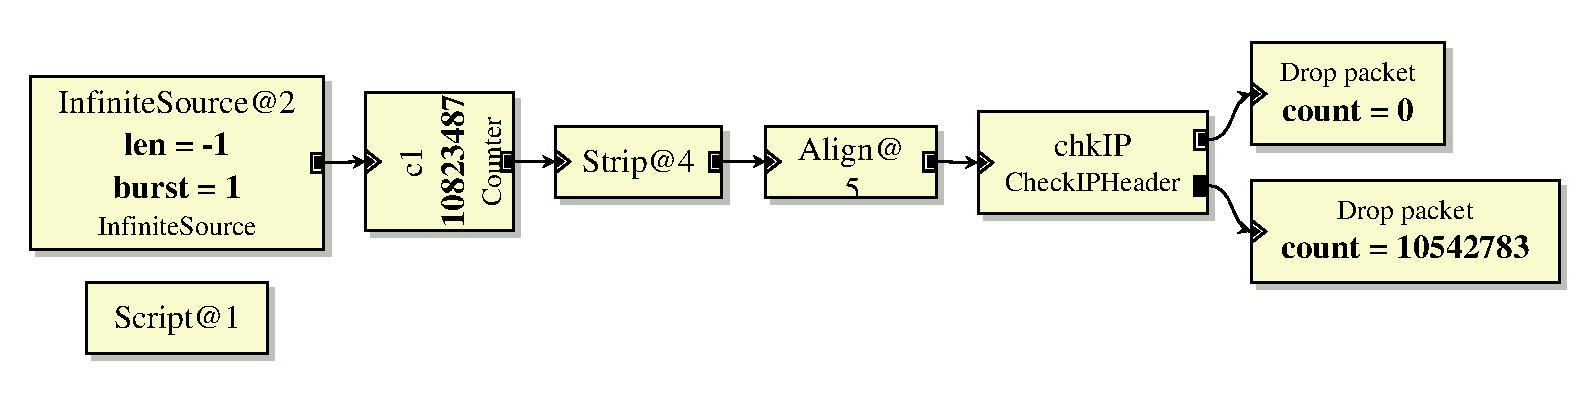
\includegraphics[scale=0.6]{counter_test.pdf}
	  \captionof{figure}{\texttt{Counter\_test} Click configuration}
	  \label{fig:countertest}
  \end{center}
  To avoid IP CRC checking, we temporarily disable CRC checking by using flag "\texttt{CHECKSUM false}" in \texttt{CheckIPHeader} element. Another solution is to use \texttt{SetIPChecksum} to repair CRC in generated IP packets. Since We can visualize the result by using clicky to replace steps that print out screen counting results from Counter elements. 
  \subsection{\texttt{RandInfiniteSource} element}
  Test RandInfiniteSource
  \subsection{\texttt{RandomQueue} element}
  Test RandomQueue
  \subsection{\texttt{Random\_IP\_generator} configuration}
  \begin{center}
	  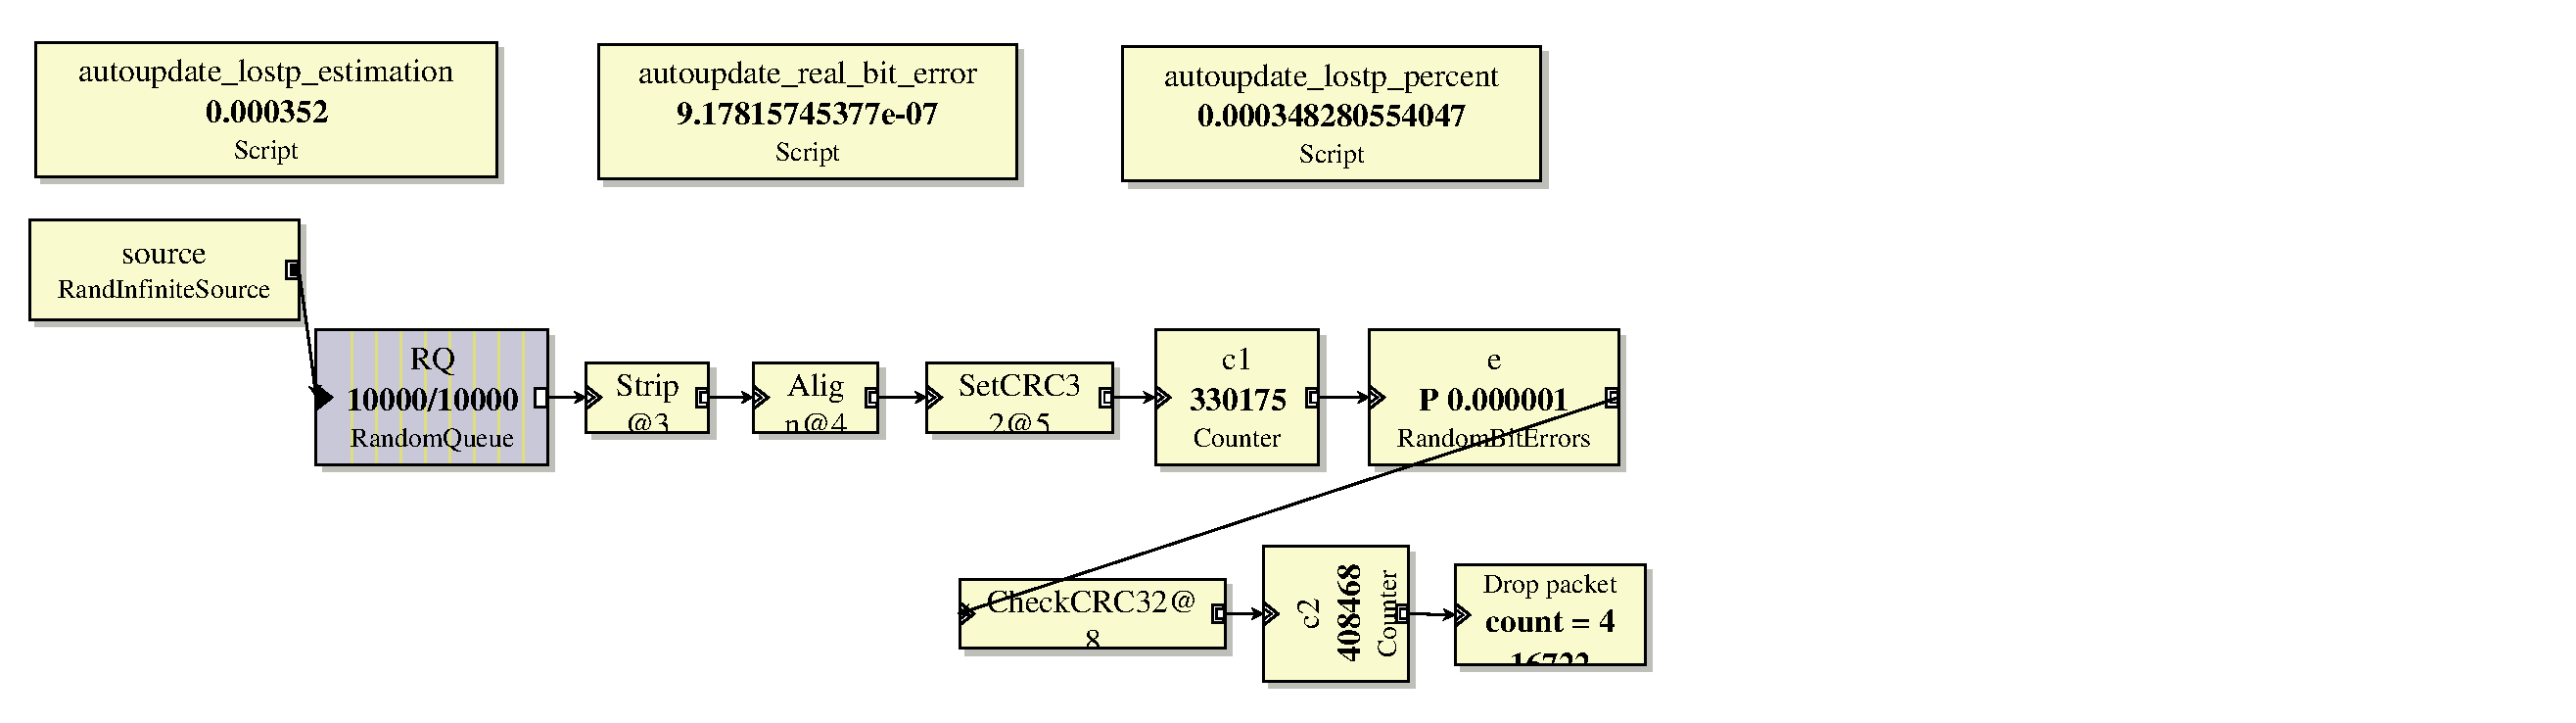
\includegraphics[scale=0.55]{Random_IP_generator.pdf}
	  \captionof{figure}{\texttt{Random\_IP\_generator} configuration}
	  \label{fig:randomipgenerator}
  \end{center}
   
  \section{TCP/UDP traffic generation}
  \subsection{TCP traffic}
  \begin{center}
	  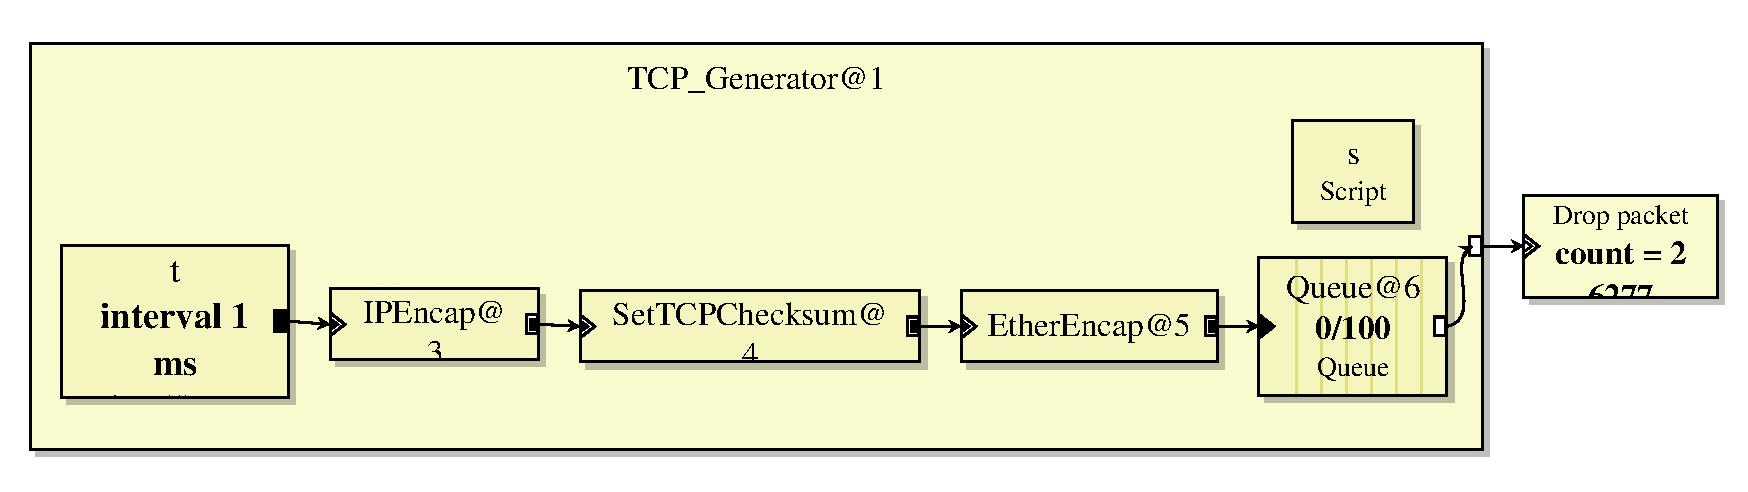
\includegraphics[scale=0.55]{TCP_Source.pdf}
	  \captionof{figure}{\texttt{TCP\_Source} element}
	  \label{fig:tcpsource}
  \end{center}
  \subsection{UDP traffic}
    \begin{center}
	  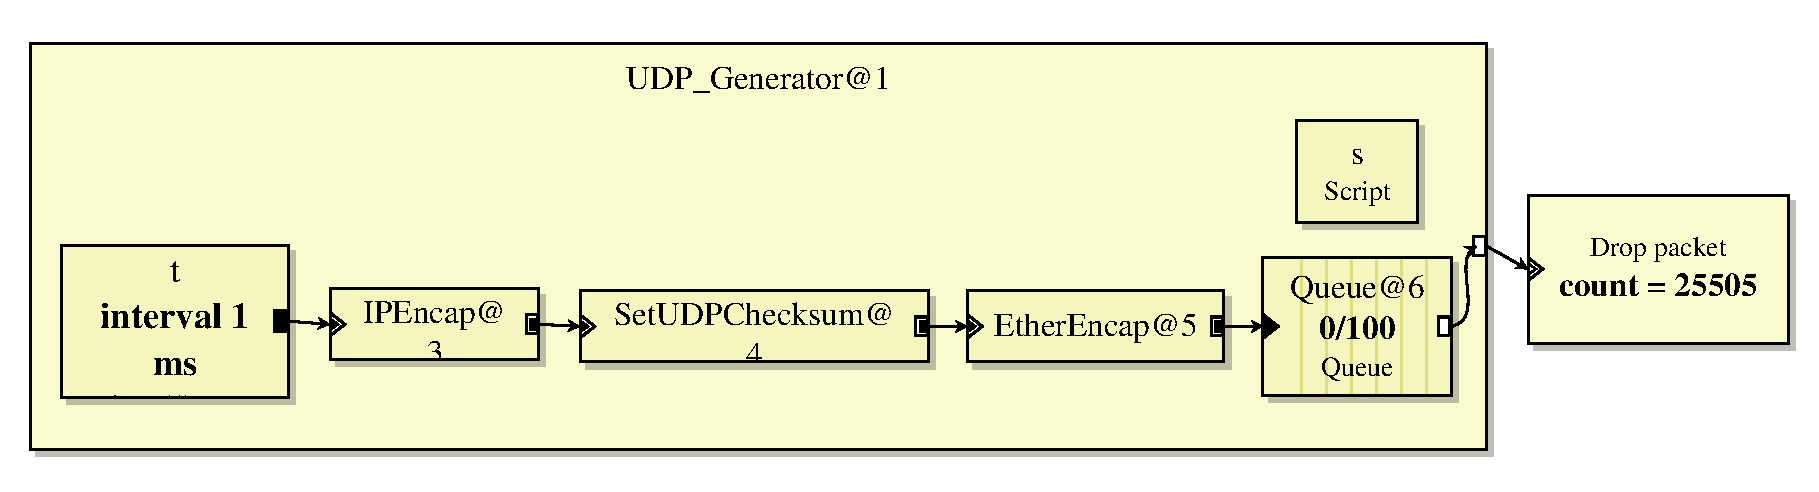
\includegraphics[scale=0.55]{UDP_Source.pdf}
	  \captionof{figure}{\texttt{UDP\_Source} element}
	  \label{fig:udpsource}
  \end{center}
  \subsection{\texttt{TCP\_UDP\_generator} element}
    \begin{center}
	  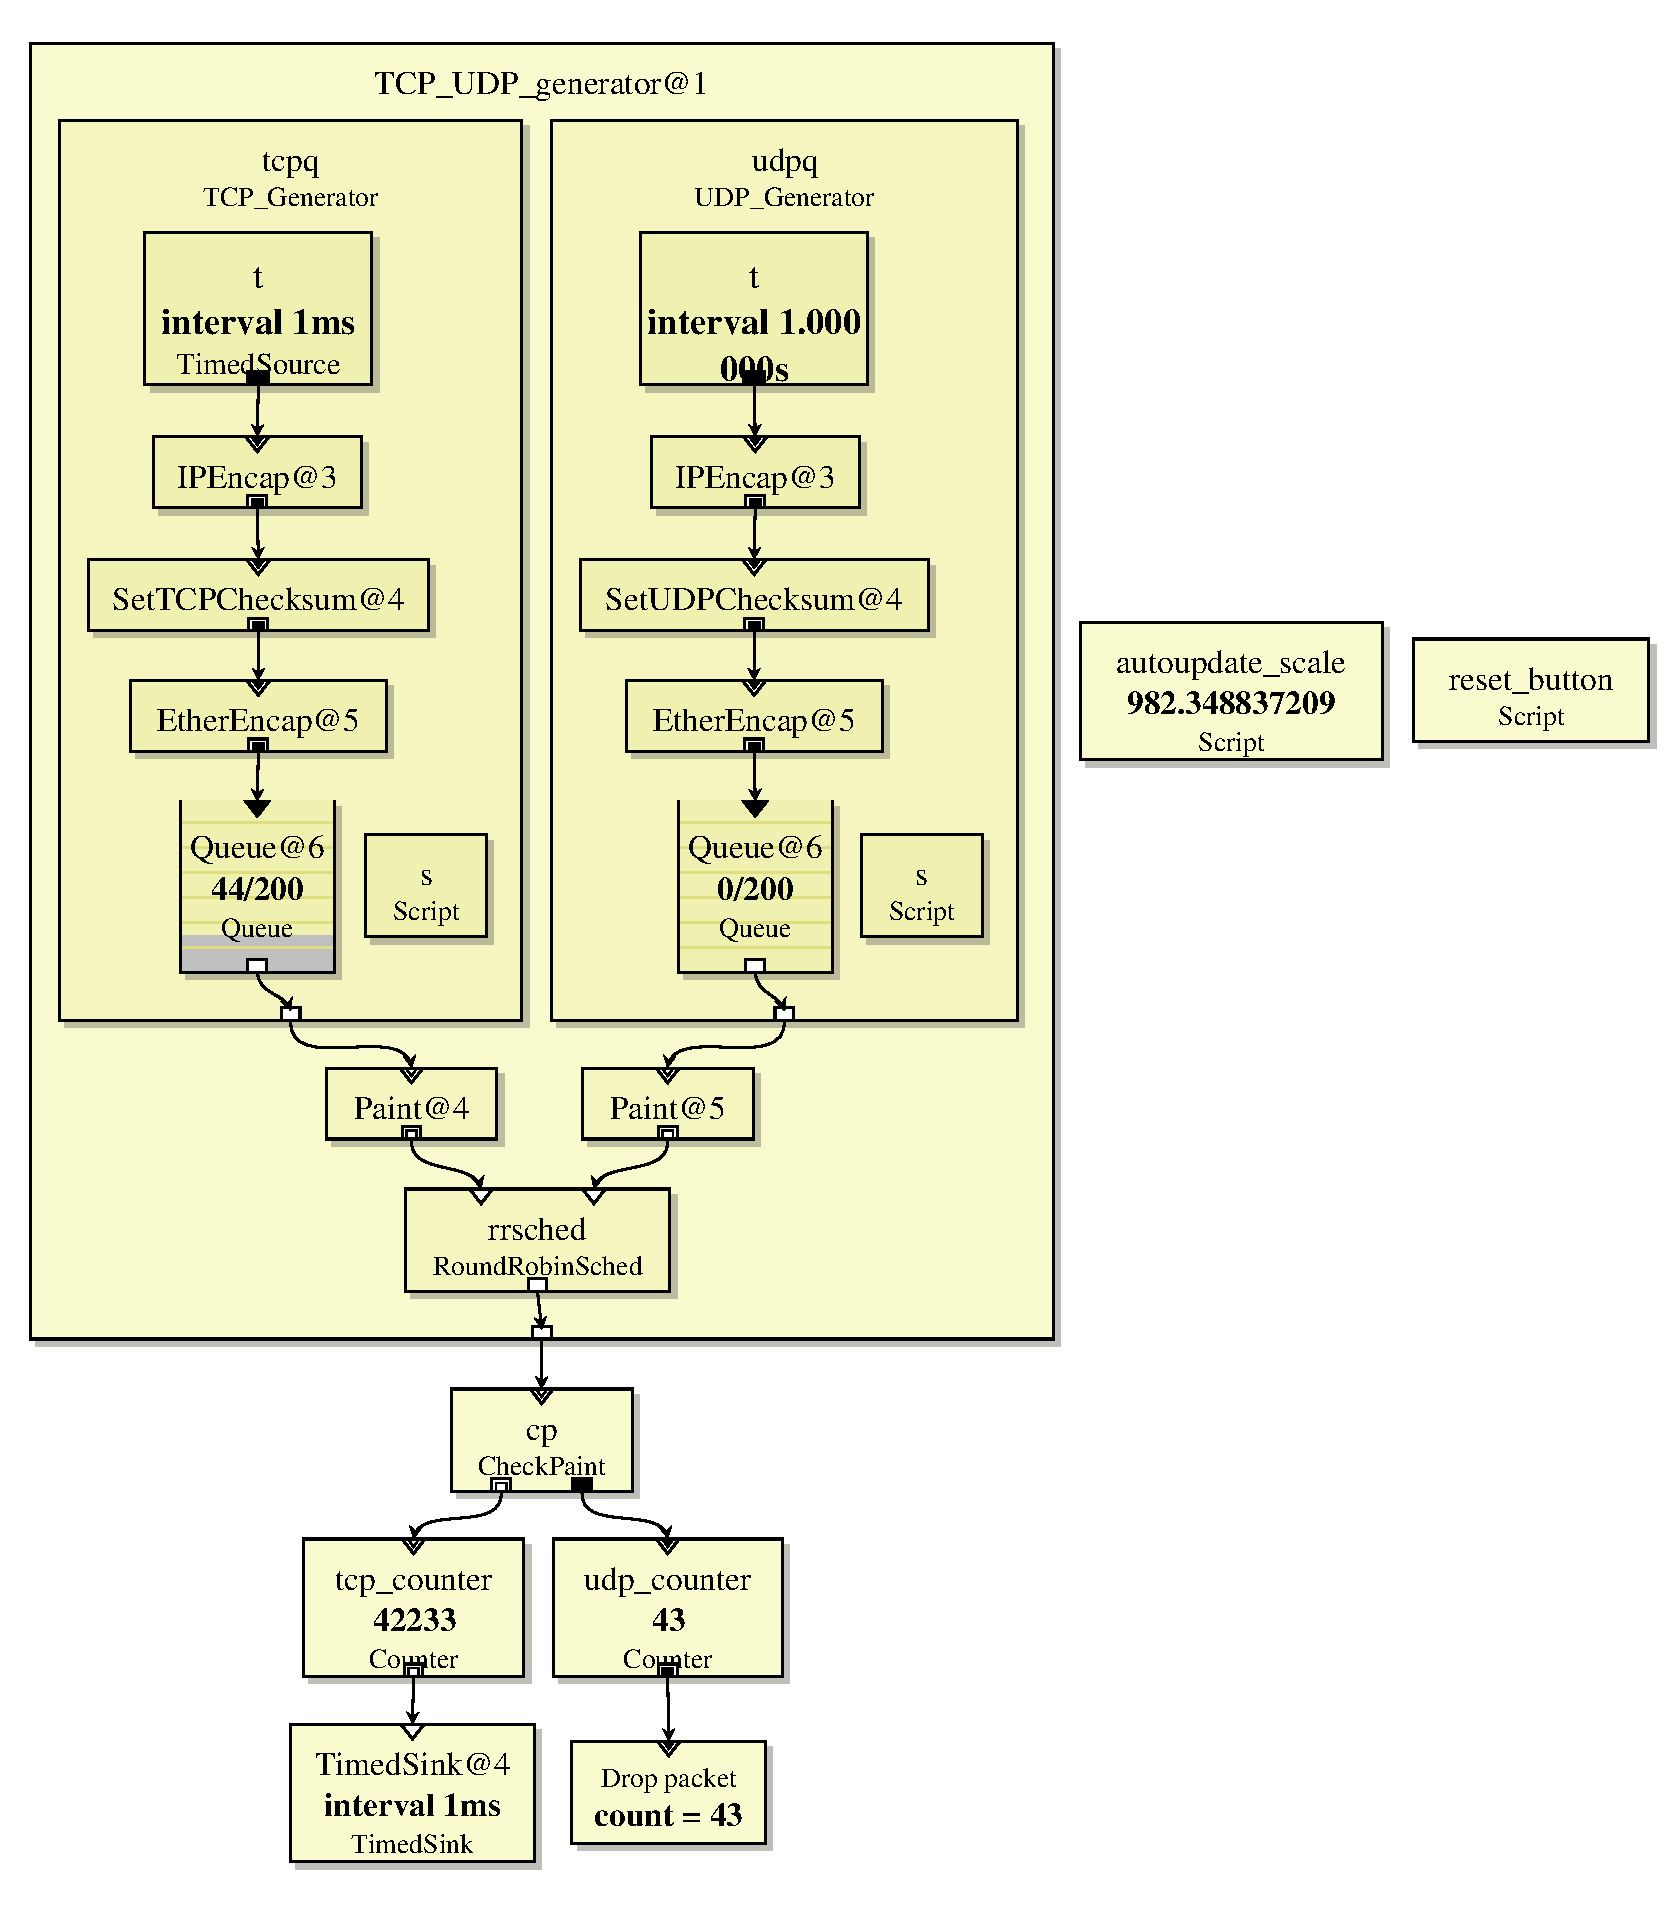
\includegraphics[scale=0.55]{TCP_UDP_generator.pdf}
	  \captionof{figure}{\texttt{TCP\_UDP\_generator} element}
	  \label{fig:tcpudp}
  \end{center}
  \section{Shapers and Policers}
  \subsection{Uncontrolled flow}
  We have tried some implementations of uncontrolled flow but the main idea is
  that the inter-time (interval) between two consecutive packets is a random
  number.
  \subsection{Leaky bucket}
  \subsection{Token bucket}
  \subsection{Cascading Leaky and Token bucket}
  \subsection{Negotiation (CIR, CBS, EBS)}
  \section{Schedulers}
  \subsection{FIFO scheduler}
  \subsection{Round Robin scheduler}
  \subsection{Weighted Round Robin Scheduler}
  \subsection{Deficit Round Robin scheduler}
  \subsection{\texttt{SetVirtualClock} element}
  \subsection{Weighted Deficit Round Robin scheduler}
  \subsection{Virtual Clock scheduler}
  \subsection{Weighted Fair Queue scheduler}
  \section{Congestion control}
    \begin{center}
	  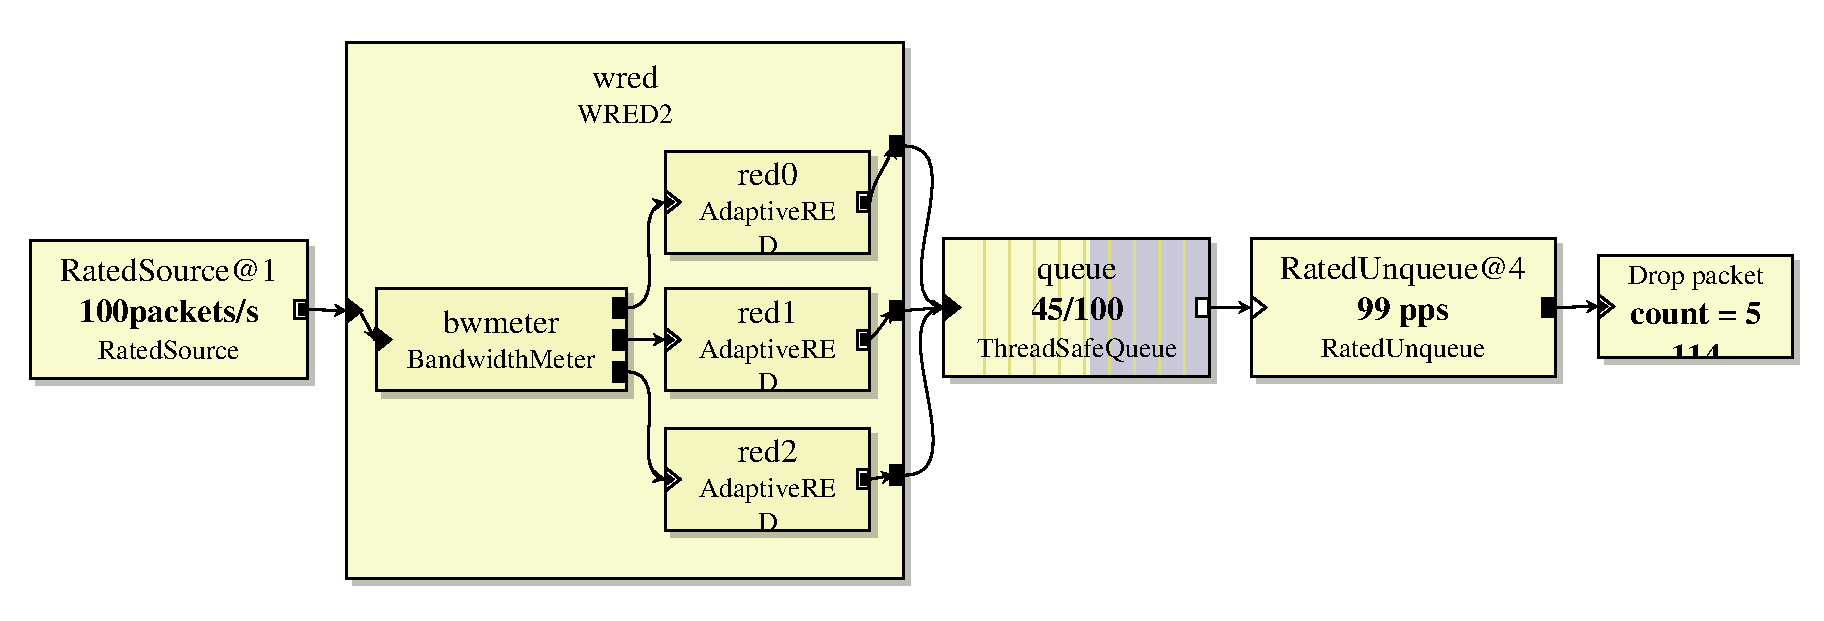
\includegraphics[scale=0.5]{wred2.pdf}
	  \captionof{figure}{One simple implementation of \texttt{WRED} element}
	  \label{fig:wred2}
    \end{center}
  
\end{document}
